\documentclass[12pt,letterpaper]{exam}
\usepackage[lmargin=1in,rmargin=1in,tmargin=1in,bmargin=1in]{geometry}
\usepackage{../style/exams}

% -------------------
% Course & Exam Information
% -------------------
\newcommand{\course}{MATH 142: Exam 1}
\newcommand{\term}{Spring --- 2025}
\newcommand{\examdate}{02/13/2025}
\newcommand{\timelimit}{75 Minutes}

\setbool{hideans}{false} % Student: True; Instructor: False

\newcommand{\boxseven}[4]{%
	\draw[thick] (0,0) -- (4,0) -- (4,4) -- (0,4) -- (0,0);
	\draw[thick] (0,2) -- (4,2);
	\draw[thick] (2,0) -- (2,4);
	% '7'
	\draw (1.7,2.2) -- (2.3,2.2) -- (1.7,1.6);
	% Entries
	\node at (1,3) {$#1$};	% u
	\node at (3,1) {$#2$};	% dv
	\node at (1,1) {$#3$};	% du
	\node at (3,3) {$#4$};	% 
}


\usetikzlibrary{calc}
\usepackage{booktabs}
\tikzset{Arrow Style/.style={text=black, font=\boldmath}}
\newcommand{\tikzmark}[1]{%
    \tikz[overlay, remember picture, baseline] \node (#1) {};%
}
\newcommand*{\XShift}{0.5em}
\newcommand*{\YShift}{0.5ex}
\NewDocumentCommand{\DrawArrow}{s O{} m m m}{%
    \begin{tikzpicture}[overlay,remember picture]
        \draw[->, thick, Arrow Style, #2] 
                ($(#3.west)+(\XShift,\YShift)$) -- 
                ($(#4.east)+(-\XShift,\YShift)$)
        node [midway,above] {#5};
    \end{tikzpicture}%
}

\usepackage{cancel}


% -------------------
% Content
% -------------------
\begin{document}

\examtitle
\instructions{Write your name on the appropriate line on the exam cover sheet. This exam contains \numpages\ pages (including this cover page) and \numquestions\ questions. Check that you have every page of the exam. Answer the questions in the spaces provided on the question sheets. Be sure to answer every part of each question and show all your work. If you run out of room for an answer, continue on the back of the page --- being sure to indicate the problem number. \par\vspace{0.3cm}

{\bfseries Choose any of the seven questions in this exam. Only these seven problems will be graded. Indicate which you \underline{do not} want to be graded by circling that problem number on this cover page.}
} 
\scores
\bottomline
\newpage


% -------------------
% Questions
% -------------------
\begin{questions}

% Question 1
\newpage
\question[10] Showing all your work, integrate the following: \par\vspace{0.3cm}
	\begin{enumerate}[(a)]
	\item $\ds\int \sin^2 \theta \;d\theta$ \par\vspace{3cm}
		\[
		\int \sin^2 \theta \;d\theta= \int \left( \dfrac{1 - \cos 2\theta}{2} \right) \;d\theta= \dfrac{1}{2} \int \left( 1 - \cos 2 \theta \right) \;d\theta= \dfrac{1}{2} \left( \theta - \dfrac{\sin 2\theta}{2} \right) + C
		\] \par\vspace{4.6cm}
	
	\item $\ds\int \dfrac{3x - 7}{x^2 + 1} \;dx$ \par\vspace{3cm}
		\[
		\int \dfrac{3x - 7}{x^2 + 1} \;dx= \int \left( \dfrac{3x}{x^2 + 1} - \dfrac{7}{x^2 + 1} \right) \;dx= \dfrac{3}{2} \ln|x^2 + 1| - 7 \arctan x + C
		\] 
	\end{enumerate}



% Question 2
\newpage
\question[10] Showing all your work, integrate the following:
	\[
	\int_0^{\pi/4} \sec^4 \theta \, \tan^3 \theta \;d\theta
	\] \pspace

{\footnotesize \itshape \tsol Let $u= \tan \theta$, so that $du= \sec^2 \theta \;d\theta$. If $\theta= 0$, then $u= \tan 0= 0$. If $\theta= \frac{\pi}{4}$, then $u= \tan \frac{\pi}{4}= 1$. Using the fact that $\sec^2 \theta= \tan^2 \theta + 1$, we have\dots
	\[
	\begin{aligned}
	\int_0^{\pi/4} \sec^4 \theta \, \tan^3 \theta \;d\theta&= \int_0^{\pi/4} \sec^2 \theta \, \tan^3 \theta \cdot \sec^2 \theta \;d\theta \\
	&= \int_0^{\pi/4} (\tan^2 \theta + 1) \, \tan^3 \theta \cdot \sec^2 \theta \;d\theta \\
	&= \int_0^1 (u^2 + 1) u^3 \;du \\
	&= \int_0^1 (u^5 + u^3) \;du \\
	&= \left( \dfrac{u^6}{6} + \dfrac{u^4}{4} \right) \bigg|_0^1 \\
	&= \left( \dfrac{1}{6} + \dfrac{1}{4} \right) - \left( \dfrac{0}{6} + \dfrac{0}{4} \right) \\
	&= \dfrac{2}{12} + \dfrac{3}{12} \\
	&= \dfrac{5}{12}
	\end{aligned}
	\]
	
	\begin{center} {\bfseries OR} \end{center}

Let $u= \sec \theta$, so that $du= \sec \theta \tan \theta \;d\theta$. If $\theta= 0$, then $u= \sec 0= 1$. If $\theta= \frac{\pi}{4}$, then $u= \sec \frac{\pi}{4}= \sqrt{2}$. Using the fact that $\tan^2 \theta= \sec^2 \theta - 1$, we have\dots
	\[
	\begin{aligned}
	\int_0^{\pi/4} \sec^4 \theta \, \tan^3 \theta \;d\theta&= \int_0^{\pi/4} \sec^3 \theta \tan^2 \theta \cdot \sec \theta \tan \theta \;d\theta \\
	&= \int_0^{\pi/4} \sec^3 \theta \, (\sec^2 \theta - 1) \cdot \sec \theta \tan \theta \;d\theta \\
	&= \int_1^{\sqrt{2}} u^3 (u^2 - 1) \;du \\
	&= \int_1^{\sqrt{2}} (u^5 - u^3) \;du \\
	&= \left( \dfrac{u^6}{6} - \dfrac{u^4}{4} \right) \bigg|_1^{\sqrt{2}} \\
	&= \left( \dfrac{\sqrt{2}^{\,6}}{6} - \dfrac{\sqrt{2}^{\,4}}{4} \right) - \left( \dfrac{1}{6} - \dfrac{1}{4} \right) \\
	&= \left( \dfrac{8}{6} - \dfrac{4}{4} \right) - \dfrac{-1}{12} \\
	&= \dfrac{16}{12} - \dfrac{12}{12} + \dfrac{1}{12} \\
	&= \dfrac{5}{12}
	\end{aligned}
	\]
}

\newpage

{
\thispagestyle{empty}
\footnotesize \itshape
	\[
	\int_0^{\pi/4} \sec^4 \theta \, \tan^3 \theta \;d\theta
	\]
Interesting enough, there are two other possibilities for approaching this integral. \pspace

Taking $u= \sec^2 \theta$, we have $du= 2 \sec \theta \cdot \sec \theta \tan \theta \;d\theta= 2 \sec^2 \theta \tan \theta \;d\theta$. We then also have bounds given by $u= \sec^2(0)= 1^2= 1$ and $u= \sec^2 \frac{\pi}{4}= (\sqrt{2})^2= 2$. Using the fact that $\tan^2 \theta= \sec^2 \theta - 1$, we have\dots
	\[
	\begin{aligned}
	\int_0^{\pi/4} \sec^4 \theta \, \tan^3 \theta \;d\theta&= \int_0^{\pi/4} \sec^2 \theta \tan^2 \theta \cdot \sec^2 \theta \tan \theta \;d\theta \\
	&= \dfrac{1}{2} \int_0^{\pi/4} \sec^2 \theta \, (\sec^2 \theta - 1) \cdot 2 \sec^2 \theta \tan \theta \;d\theta \\
	&= \dfrac{1}{2} \int_1^{2} u \, (u - 1) \;du \\
	&= \dfrac{1}{2} \int_1^2 (u^2 - u) \;du \\
	&= \dfrac{1}{2} \left[ \dfrac{u^3}{3} - \dfrac{u^2}{2} \right] \bigg|_1^2 \\
	&= \dfrac{1}{2} \left[ \left( \dfrac{8}{3} - \dfrac{4}{2} \right) - \left( \dfrac{1}{3} - \dfrac{1}{2} \right) \right] \\
	&= \dfrac{1}{2} \left[ \dfrac{2}{3} - \left(-\dfrac{1}{6} \right) \right] \\
	&= \dfrac{1}{2} \cdot \dfrac{5}{6} \\
	&= \dfrac{5}{12}
	\end{aligned}
	\] 
We can also choose $u= \tan^2 \theta$, which implies that $du= 2 \tan \theta \cdot \sec^2 \theta \;d\theta$. The bounds are then $u= \tan^2(0)= 0^2= 0$ and $u= \tan^2 \frac{\pi}{4}= 1^2= 1$. Using the fact that $\sec^2 \theta= \tan^2 \theta + 1$, we have\dots
	\[
	\begin{aligned}
	\int_0^{\pi/4} \sec^4 \theta \, \tan^3 \theta \;d\theta&= \int_0^{\pi/4} \sec^2 \theta \tan^2 \theta \cdot \tan \theta \sec^2 \theta \;d\theta \\
	&= \dfrac{1}{2} \int_0^{\pi/4} (\tan^2 \theta + 1) \tan^2 \theta \cdot 2 \tan \theta \sec^2 \theta \;d\theta \\
	&= \dfrac{1}{2} \int_0^1 (u + 1) u \;du \\
	&= \dfrac{1}{2} \int_0^1 (u^2 + u) \;du \\
	&= \dfrac{1}{2} \left[ \dfrac{u^3}{3} + \dfrac{u^2}{2} \right] \bigg|_0^1 \\
	&= \dfrac{1}{2} \left[ \left( \dfrac{1}{3} + \dfrac{1}{2} \right) - \left( 0 + 0 \right) \right] \\
	&= \dfrac{1}{2} \left[ \dfrac{5}{6} - 0 \right] \\
	&= \dfrac{5}{12}
	\end{aligned}
	\]

\setcounter{page}{3}
}



% Question 3
\newpage
\question[10] Showing all your work, integrate the following:
	\[
	\int \dfrac{dx}{\sqrt{x^2 - 9}}
	\] \pspace

{\itshape \tsol We know from the Pythagorean Theorem that $a^2 + b^2= c^2$, which implies that $a^2= c^2 - b2$. Taking $c^2= x^2$, i.e. $c= x$, and $b^2= 9$, i.e. $b= 3$, we have $a^2= c^2 - b^2= x^2 - 9$. This also shows that $a= \sqrt{x^2 - 9}$. There are two possible right triangles corresponding to these sides we could draw:
	\[
	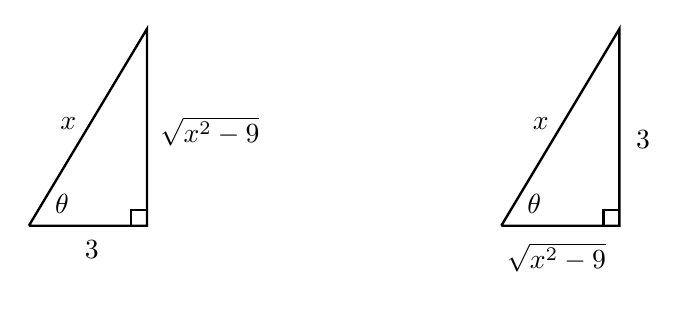
\begin{tikzpicture}
	\draw[line width=0.03cm] (0,0) -- (1.5,0) -- (1.5,2.5) -- (0,0);
	\draw[line width=0.03cm] (1.3,0) -- (1.3,0.2) -- (1.5,0.2);
	\node at (0.8,-0.3) {$3$};
	\node at (2.3,1.2) {$\sqrt{x^2 - 9}$};
	\node at (0.5,1.3) {$x$};
	\node at (0.42,0.28) {$\theta$};
	
	\tikzset{shift={(6,0)}};

	\draw[line width=0.03cm] (0,0) -- (1.5,0) -- (1.5,2.5) -- (0,0);
	\draw[line width=0.03cm] (1.3,0) -- (1.3,0.2) -- (1.5,0.2);
	\node at (1.8,1.1) {$3$};
	\node at (0.7,-0.4) {$\sqrt{x^2 - 9}$};
	\node at (0.5,1.3) {$x$};
	\node at (0.42,0.28) {$\theta$};
	\end{tikzpicture}
	\]
Using the right triangle on the left, we have $\cos \theta= \frac{3}{x}$, so that $x= \frac{3}{\cos \theta}= 3 \sec \theta$. But then $dx= 3 \sec \theta \tan \theta \;d\theta$. Observe that $\tan \theta= \frac{\sqrt{x^2 - 9}}{3}$, so that $\sqrt{x^2 - 9}= 3 \tan \theta$. But then\dots
	\[
	\int \dfrac{dx}{\sqrt{x^2 - 9}}= \int \dfrac{3 \sec \theta \tan \theta}{3 \tan \theta} \;d\theta= \int \sec \theta \;d\theta= \ln| \sec \theta + \tan \theta| + C
	\]
But we know that $\sec \theta= \frac{x}{3}$ and $\tan \theta= \frac{\sqrt{x^2 - 9}}{3}$. Therefore, 
	\[
	\int \dfrac{dx}{\sqrt{x^2 - 9}}= \ln| \sec \theta + \tan \theta| + C= \ln\left| \dfrac{x}{3} + \dfrac{\sqrt{x^2 - 9}}{3} \right| + C
	\] \pspace
Alternatively, using the right triangle on the right, we have $\sin \theta= \frac{3}{x}$, so that $x= \frac{3}{\sin \theta}= 3 \csc \theta$. But then $dx= -3 \csc \theta \cot \theta$. Observe that $\tan \theta= \frac{3}{\sqrt{x^2 - 9}}$, so that $\sqrt{x^2 - 9}= \frac{3}{\tan \theta}= 3 \cot \theta$. But then\dots
	\[
	\int \dfrac{dx}{\sqrt{x^2 - 9}}= \int \dfrac{-3 \csc \theta \cot \theta}{3 \cot \theta} \;d\theta= -\int \csc \theta \;d\theta= -\ln| \csc \theta - \cot \theta| + C
	\]
But we know that $\csc \theta= \frac{x}{3}$ and $\cot \theta= \frac{\sqrt{x^2 - 9}}{3}$. Therefore, 
	\[
	\int \dfrac{dx}{\sqrt{x^2 - 9}}= -\ln| \csc \theta - \cot \theta| + C= -\ln| \csc \theta - \cot \theta| + C= -\ln \left| \dfrac{x}{3} - \dfrac{\sqrt{x^2 - 9}}{3} \right| + C
	\]

\vfill {\tiny Note. Observing that $\ln(\frac{1}{3})$ is a constant, we can write the solution as $\ln\left| \frac{x}{3} \pm \dfrac{\sqrt{x^2 - 9}}{3} \right| + C= \ln\left| \frac{1}{3} \left( x \pm \sqrt{x^2 - 9} \right) \right| + C= \ln(\frac{1}{3}) + \ln\left| x \pm \sqrt{x^2 - 9} \right| + C= \ln\left| x \pm \sqrt{x^2 - 9} \right| + C$. Furthermore, to see that the solutions are equivalent, observe that by `rationalizing', we have $-\ln|x - \sqrt{x^2 - 9}|= \ln| (x - \sqrt{x^2 - 9})^{-1}|= \ln| \frac{1}{9} (x + \sqrt{x^2 - 9})|= \ln(\frac{1}{9}) + \ln| x + \sqrt{x^2 - 9}|$. Therefore, the solutions differ only by a constant. One could also have integrated $\csc \theta$ using the antiderivative $-\ln| \csc \theta + \cot \theta| + C$, which used in the integral above results in the same solution as using the substitution $x= 3 \sec \theta$.}
}



% Question 4
\newpage
\question[10] Showing all your work, integrate the following:
	\[
	\int_0^4 \dfrac{dx}{\sqrt{4 - x}}
	\] \pspace

{\itshape \tsol Observe that $\frac{1}{\sqrt{4 - x}}$ is undefined at $x= 4$, so that $\frac{1}{\sqrt{4 - x}}$ is not continuous at $x= 4$. Therefore, this is an improper integral. We first find the indefinite integral:
	\[
	\int \dfrac{dx}{\sqrt{4 - x}}= \int (4 - x)^{-1/2} \;dx= (4 - x)^{1/2} \cdot \dfrac{1}{\frac{1}{2}} \cdot \dfrac{1}{-1}= -2 \sqrt{4 - x} + C
	\]
But then, we have\dots
	\[
	\begin{aligned}
	\int_0^4 \dfrac{dx}{\sqrt{4 - x}}&:= \lim_{b \to 4^-} \int_0^b \dfrac{dx}{\sqrt{4 - x}} \\[0.3cm]
	&= \lim_{b \to 4^-} -2 \sqrt{4 - x} \bigg|_{0}^b \\[0.3cm]
	&= -2 \lim_{b \to 4^-} \sqrt{4 - x} \bigg|_{0}^b \\[0.3cm]
	&= -2 \left( \lim_{b \to 4^-} \sqrt{4 - b} - \sqrt{4 - 0} \right) \\[0.3cm]
	&= -2 \left( \sqrt{0} - \sqrt{4} \right) \\[0.3cm]
	&= -2 \cdot -2 \\[0.3cm]
	&= 4
	\end{aligned}
	\] \vfill

{
\scriptsize Note. To compute $\int \frac{dx}{\sqrt{4 - x}}$, one needs the $u$-substitution $u= 4 - x$, which implies $du= -dx$. Then $\int \frac{dx}{\sqrt{4 - x}}= \int \frac{-du}{\sqrt{u}}= \int -u^{-1/2} \;du= -2u^{1/2} + C= -2 \sqrt{4 - x}+ C$. Interestingly, one can also choose $u= \sqrt{4 - x}$. This implies that $du= \frac{-1}{2\sqrt{4 - x}} \;dx= \frac{-1}{2u} \;dx$, i.e. $dx= -2u \;du$. But then $\int \frac{dx}{\sqrt{4 - x}}= \int \frac{-2u}{u} \;du= -2 \int \;du= -2u + C= -2\sqrt{4 - x} + C$. One could also integrate this using trig substitution: construct the triangle given below. One then has $\sin \theta= \frac{\sqrt{x}}{2}$, so that $\sqrt{x}= 2 \sin \theta$. But then $x= 4 \sin^2 \theta$, so that $dx= 8 \sin \theta \cdot \cos \theta \;d\theta$. Observe that $\cos \theta= \frac{\sqrt{4 - x}}{2}$, which implies $\sqrt{4 - x}= 2 \cos \theta$. But then $\int \frac{dx}{\sqrt{4 - x}}= \int \frac{8 \sin \theta \cos \theta}{2 \cos \theta} \;d\theta= 4 \int \sin \theta \;d\theta= -4 \cos \theta + C= -4 \cdot \frac{\sqrt{4 - x}}{2} + C= -2 \sqrt{4 - x} + C$. 
	\[
	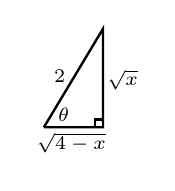
\begin{tikzpicture}[scale=0.5]
	\draw[line width=0.03cm] (0,0) -- (1.5,0) -- (1.5,2.5) -- (0,0);
	\draw[line width=0.03cm] (1.3,0) -- (1.3,0.2) -- (1.5,0.2);
	\node at (0.7,-0.4) {\scriptsize$\sqrt{4 - x}$};
	\node at (2.0,1.2) {\scriptsize$\sqrt{x}$};
	\node at (0.4,1.3) {\scriptsize$2$};
	\node at (0.5,0.32) {\scriptsize$\theta$};
	\end{tikzpicture}
	\]
}
}



% Question 5
\newpage
\question[10] Showing all your work, integrate the following:
	\[
	\int x^3 e^{2x} \;dx
	\] \pspace

{\itshape \tsol Using tabular integration, we have\dots
	\[
	\begin{array}{c @{\hspace*{1.3cm}} c} \toprule
	u & dv \\ \cmidrule(lr){1-2}
	x^3 \tikzmark{Left 1} & \tikzmark{Right 1} e^{2x} \\[0.3cm]
	3x^2 \tikzmark{Left 2} & \tikzmark{Right 2} \frac{1}{2} \, e^{2x} \\[0.3cm]
	6x \tikzmark{Left 3} & \tikzmark{Right 3} \frac{1}{4} \, e^{2x} \\[0.3cm]
	6 \tikzmark{Left 4} & \tikzmark{Right 4} \frac{1}{8} \, e^{2x} \\[0.3cm]
	0 \tikzmark{Left 5} & \tikzmark{Right 5} \frac{1}{16} \, e^{2x} 
	
	\DrawArrow{Left 1}{Right 2}{+}
	\DrawArrow{Left 2}{Right 3}{--}
	\DrawArrow{Left 3}{Right 4}{+}
	\DrawArrow{Left 4}{Right 5}{--}
	\end{array}
	\]
Therefore, we have\dots
	\[
	\begin{aligned}
	\int x^3 e^{2x} \;dx&= \dfrac{1}{2}\, x^3 e^{2x} - \dfrac{3}{4}\, x^2 e^{2x} + \dfrac{6}{8}\, x e^{2x} - \dfrac{6}{16} e^{2x} + C \\[0.3cm]
	&= \dfrac{1}{2}\, x^3 e^{2x} - \dfrac{3}{4}\, x^2 e^{2x} + \dfrac{3}{4}\, x e^{2x} - \dfrac{3}{8}\, e^{2x} + C \\
	\end{aligned}
	\]
\vfill

{\tiny Note. We can also express the answer as $\ds\int x^3 e^{2x} \;dx= e^{2x} \left( \frac{1}{2}\, x^3 - \frac{3}{4}\, x^2 + \frac{3}{4}\, x - \frac{3}{8} \right) + C= \dfrac{e^{2x}}{8} \, \left( 4x^3 - 6x^2 + 6x - 3 \right) + C$.}
}



% Question 6
\newpage
\question[10] Showing all your work, integrate the following:
	\[
	\int e^{x} \cos(2x) \;dx
	\]

{\itshape \tsol Using a modified tabular integration, we have\dots
	\[
	\begin{array}{c @{\hspace*{1.3cm}} c} \toprule
	u & dv \\ \cmidrule(lr){1-2}
	\cos(2x) \tikzmark{Left 1} & \tikzmark{Right 1} e^x \\[0.5cm]
	-2 \sin(2x) \tikzmark{Left 2} & \tikzmark{Right 2} e^x \\[0.3cm]
	-4 \cos(2x) \tikzmark{Left 3}  & \tikzmark{Right 3} e^x 
	
	\DrawArrow{Left 1}{Right 2}{+}
	\DrawArrow{Left 2}{Right 3}{--}
	\DrawArrow{Left 3}{Right 3}{\!\!\!\!\!$\phantom{}_{\genfrac{}{}{0pt}{}{}{+}}$}
	\end{array}
	\]
But then, we have\dots
	\[
	\begin{gathered}
	\int e^{x} \cos(2x) \;dx= e^x \cos(2x) + 2 e^x \sin(2x) - \int 4 e^x \cos(2x) \;dx \\[0.3cm]
	\int e^{x} \cos(2x) \;dx= e^x \cos(2x) + 2 e^x \sin(2x) - 4 \int e^x \cos(2x) \;dx \\[0.3cm]
	5 \int e^{x} \cos(2x) \;dx= e^x \cos(2x) + 2 e^x \sin(2x) + C \\[0.3cm]
	\int e^{x} \cos(2x) \;dx= \dfrac{1}{5} \left( e^x \cos(2x) + 2 e^x \sin(2x) \right) + C
	\end{gathered}
	\]
\vfill
{\tiny Note. We can also express the answer as $\int e^{x} \cos(2x) \;dx= \dfrac{e^x}{5} \left( \cos(2x) + 2 \sin(2x) \right) + C$.}
}



% Question 7
\newpage
\question[10] Showing all your work, integrate the following:
	\[
	\int_1^e \dfrac{\ln x}{x^2} \;dx
	\]

{\itshape \tsol Using LIATE, we choose $u= \ln x$, which forces $dv= \dfrac{1}{x^2}$. But then we have\dots
	\[
	\begin{tikzpicture}
	\boxseven{\ln x}{\dfrac{1}{x^2}}{\dfrac{1}{x}}{-\dfrac{1}{x}}
	\end{tikzpicture}
	\]
Therefore, we have\dots
	\[
	\begin{aligned}
	\int_1^e \dfrac{\ln x}{x^2} \;dx&= -\dfrac{\ln x}{x} \bigg|_1^e - \int_1^e \dfrac{-1}{x^2} \;dx \\[0.3cm]
	&= \left( -\dfrac{\ln e}{e} - \dfrac{-\ln 1}{1} \right) + \int_1^e \dfrac{dx}{x^2} \\[0.3cm]
	&= \left(-\dfrac{1}{e} - 0 \right) + \dfrac{-1}{x} \bigg|_1^e \\[0.3cm]
	&= -\dfrac{1}{e} + \left( \dfrac{-1}{e} - \dfrac{-1}{1} \right) \\[0.3cm]
	&= -\dfrac{1}{e} - \dfrac{1}{e} + 1 \\[0.3cm]
	&= -\dfrac{2}{e} + 1 \\[0.3cm]
	&= 1 - \dfrac{2}{e}
	\end{aligned}
	\]
\vfill
{\tiny Note. Using a common denominator, we can express this answer as $1 - \frac{2}{e}= \frac{e}{e} - \frac{2}{e}= \frac{e - 2}{e}$.}
}



% Question 8
\newpage
\question[10] Showing all your work, integrate the following:
	\[
	\int \dfrac{x^2 + 5x + 6}{(x - 1)(x + 1)^2} \;dx
	\] \pspace

{\footnotesize \itshape \tsol Observe that the degree of the denominator, which is 3, is strictly larger than the degree of the top, which is 2. We can then find the partial fraction decomposition of the integrand.
	\[
	\dfrac{x^2 + 5x + 6}{(x - 1)(x + 1)^2}= \dfrac{A}{x - 1} + \dfrac{B}{x + 1} + \dfrac{C}{(x + 1)^2}
	\]
Using the original common denominator, we have\dots
	\[
	\begin{aligned}
	\dfrac{x^2 + 5x + 6}{(x - 1)(x + 1)^2}&= \dfrac{A}{x - 1} + \dfrac{B}{x + 1} + \dfrac{C}{(x + 1)^2} \\
	&= \dfrac{A(x + 1)^2 + B(x - 1)(x + 1) + C(x - 1)}{(x - 1)(x + 1)^2} \\
	&= \dfrac{A(x^2 + 2x + 1) + B(x^2 - 1) + C(x - 1)}{(x - 1)(x + 1)^2} \\
	&= \dfrac{Ax^2 + 2Ax + A + Bx^2 - B + Cx - C}{(x - 1)(x + 1)^2} \\
	&= \dfrac{(A + B)x^2 + (2A + C)x + (A - B - C)}{(x - 1)(x + 1)^2}
	\end{aligned}
	\]
Equating the numerators and relating coefficients, we have\dots \par
	\begin{table}[!ht]
	\centering
	\begin{tabular}{ll}
	$x^2 \colon$ & $1= A + B$ \\
	$x \colon$ & $5= 2A + C$ \\
	$1 \colon$ & $6= A - B - C$
	\end{tabular}
	\end{table} \par
From the last equation, we have $C= A - B - 6$. But using this in the second equation, we have $5= 2A + C= 2A + A - B - 6= 3A - B - 6$. This implies that $11= 3A - B$. Adding this to the first equation, we find that $12= 4A$, which implies that $A= 3$. But because $1= A + B= 3 + B$, we know that $B= -2$. Finally, we know that $C= A - B - 6= 3 - (-2) - 6= -1$. Alternatively, we can use Heaviside's/Cover-Up Method to find both $A$ and $C$:
	\[
	\begin{aligned}
	A&= \left. \dfrac{x^2 + 5x + 6}{\cancel{\boxed{(x - 1)}} (x + 1)^2}\, \right|_{x=1}= \dfrac{1^2 + 5(1) + 6}{(1 + 1)^2}= \dfrac{12}{4}= 3 \\
	C&= \left. \dfrac{x^2 + 5x + 6}{(x - 1) \cancel{\boxed{(x + 1)^2}}}\, \right|_{x=1}= \dfrac{(-1)^2 + 5(-1) + 6}{-1 - 1}= \dfrac{2}{-2}= -1
	\end{aligned}
	\]
One could then use any $x$-value (other than $x= \pm 1$) to find the value of $B$. For instance, using $x= 0$, we know that $\frac{x^2 + 5x + 6}{(x - 1)(x + 1)^2}= \frac{0 + 0 + 6}{-1 \cdot 1}= -6$ and $\frac{3}{0 - 1} + \dfrac{B}{0 + 1} + \frac{-1}{(0 + 1)^2}= -3 + B - 1= B - 4$. But then $B - 4= -6$ so that $B= -2$. In any case, we then have\dots
	\[
	\begin{aligned}
	\int \dfrac{x^2 + 5x + 6}{(x - 1)(x + 1)^2} \;dx&= \int \dfrac{3}{x - 1} + \dfrac{-2}{x + 1} + \dfrac{-1}{(x + 1)^2} \; dx \\[0.3cm]
	&= 3 \ln|x - 1| - 2 \ln|x + 1| + \dfrac{1}{x + 1} + K 
	\end{aligned}
	\]
}

\end{questions}
\end{document}